
%(BEGIN_QUESTION)
% Copyright 2006, Tony R. Kuphaldt, released under the Creative Commons Attribution License (v 1.0)
% This means you may do almost anything with this work of mine, so long as you give me proper credit

Regn ut trykket på utløpet av dette røret ($P_2$), om en antar at det strømmer vann ($\rho = 998.19$) og at strømningen skjer uten friksjon.(en får ikke trykktap som følge av friksjon mot rørveggen).  


$$\includegraphics[width=15.5cm]{i00450x01.eps}$$

\vskip 10pt

\noindent
{\bf Bernoulli's equation:}

$$z_1 \rho g + {v_1^2 \rho \over 2} + P_1 = z_2 \rho g + {v_2^2 \rho \over 2} + P_2$$

\vskip 20pt \vbox{\hrule \hbox{\strut \vrule{} {\bf Suggestions for Socratic discussion} \vrule} \hrule}

\begin{itemize}
\item{} One way students commonly fail to arrive at the correct answers with Bernoulli's Law calculations is by using incompatible units of measurement.  Show how all the units of measurement provided to you in this question are compatible in their given forms, with no need for conversion.
\end{itemize}

\underbar{file i00450}
%(END_QUESTION)





%(BEGIN_ANSWER)

$P_2$ = 31.39 kPa           

\vskip 10pt

It is tempting to alter Bernoulli's Equation to handle measurements in inches rather than feet (especially the annoying unit of pressure measurement: pounds per square {\it foot}, rather than PSI).  However, caution must be exercised when attempting this, because there is more to it than simply converting feet into inches every place you see ``ft'' in the equation.

$$z_1 \rho g + {v_1^2 \rho \over 2} + P_1 = z_2 \rho g + {v_2^2 \rho \over 2} + P_2$$

There is the unit of ``feet'' lurking inside the unit of ``slugs'' which must also be accounted for.  Here is the standard weight-mass-gravity equation relating slugs to pounds:

$$W = mg$$

$$[\hbox{lb}] = [\hbox{slug}] \left[ \hbox{ft} \over \hbox{s}^2 \right]$$

If we re-write the unit analysis equation to show slugs as a compound unit, we see that ``feet'' lurks within:

$$[\hbox{lb}] = \left[{\hbox{lb} \cdot \hbox{s}^2} \over \hbox{ft}\right] \left[ \hbox{ft} \over \hbox{s}^2 \right]$$

Thus, expressing $g$ in inches per second squared would require us to invent a new unit of mass (lb $\cdot$ s$^{2}$ per in) instead of slugs (lb $\cdot$ s$^{2}$ per ft).

%(END_ANSWER)





%(BEGIN_NOTES)


%INDEX% Physics, dynamic fluids: Bernoulli's equation

%(END_NOTES)


